برای حل این سوال کد زیر را استفاده می‌کنیم و آنرا تکه به تکه توضیح می‌دهیم.
ابتدا در خطوط ۳۳۴ تا ۳۳۷ به صورت کلی کد را مشاهده می‌کنیم که در ابتدا درخت را تبدیل به یک تعدادی تسک قابل مستقل از هم می‌کند، در قسمت بعدی آن تسک‌ها را با 
EDF 
زمان‌بندی می‌کند و در نهایت 
\lr{Gantt Chart}
آنها را رسم می‌کند.
\begin{latin}
    \begin{lstlisting}[language=python,style=mystyle]
def schedule_tree(tree: dict):
    turn_to_EDF(tree=tree)
    table = schedule_EDF(table=tree)
    draw_chart(table)
    \end{lstlisting}
\end{latin}
حال باقی قسمت‌های کد را تحلیل می‌کنیم.
در خطوط ۲۶۱ تا ۲۶۳ مشاهده می‌کنیم که تابع 
\lr{turn\_to\_EDF} 
در ابتدا  
\lr{Release Time}ها 
را طبق الگوریتم گفته شده در کلاس تغییر می‌دهد و سپس 
ددلاین‌ها را تغییر می‌دهد.
\begin{latin}
    \begin{lstlisting}[language=python,style=mystyle]
def turn_to_EDF(tree: dict) -> dict:
    modify_release_times(tree)
    modify_deadlines(tree)
    \end{lstlisting}
\end{latin}

حال در تابع اول ریلیز تایم‌ها را مطابق کد زیر 
عوض می‌کنیم که در خطوط ۸ و ۹ کد زیر قابل مشاهده است و برای هر اپدیت باید با 
توجه به پدران هر node 
تا جایی ریلیز را جلو ببریم که حداقل کار پدران وی 
تمام شده باشد. 
پس از اولین node 
های بدون پدر شروع می‌کنیم و آنها را وارد استک می‌کنیم 
و در هر مرحله چک می‌کنیم که راسی را وارد استک کنیم 
که تمامی پدران آن visit 
شده‌اند.

\begin{latin}
    \begin{lstlisting}[language=python,style=mystyle]
def modify_release_times(tree: dict):
    stack = list({k: v for k, v in tree.items() if not v['Fathers']}.keys())
    visited_list = []
    while len(stack) > 0:
        node = stack.pop(0)
        new_release_time = tree[node]["Release_time"]
        for father_node in tree[node]["Fathers"]:
            new_release_time = max(new_release_time, 
            tree[father_node]["Release_time"] + tree[father_node]["Computation_time"])
        tree[node]["Release_time"] = new_release_time
        visited_list.append(node)
        for child in tree[node]["Children"]:
            add = True
            for father in tree[child]["Fathers"]:
                if father not in visited_list:
                    add = False
                    break
            if add:
                stack.append(child)
    \end{lstlisting}
\end{latin}

در قسمت بعدی باید ددلاین‌ها را نیز تغییر دهیم به این صورت که 
هر ددلاین باید تا جایی عقب بیاید 
که تمامی فرزندان آن راس 
بتوانند بدون رد کردن ددلاین خود کار را انجام دهند.
پس از رئوس پایینی شروع می‌کنیم و به بالای درخت می‌آییم و 
در هر مرحله ددلاین‌ها را اپدیت می‌کنیم که در قسمت زیر قابل مشاهده است.

\begin{latin}
    \begin{lstlisting}[language=python,style=mystyle]
def modify_deadlines(tree: dict):
    stack = list({k: v for k, v in tree.items() if not v['Children']}.keys())
    visited_list = []
    while len(stack) > 0:
        node = stack.pop(0)
        new_deadline = tree[node]["Deadline"]
        for child_node in tree[node]["Children"]:
            new_deadline = min(new_deadline, tree[child_node]["Deadline"]
                                - tree[child_node]["Computation_time"])
        tree[node]["Deadline"] = new_deadline
        visited_list.append(node)
        for father in tree[node]["Fathers"]:
            add = True
            for child in tree[father]["Children"]:
                if child not in visited_list:
                    add = False
                    break
            if add:
                stack.append(father)
    \end{lstlisting}
\end{latin}

پس از این عملیات تسک‌های ما آماده‌اند که طبق 
EDF 
زمان‌بندی شوند.
پس یک زمان‌بند درست می‌کنیم که در هر مرحله 
واحد زمانی را یک واحد به جلو می‌برد و چک می‌کند که 
نزدیک‌ترین ددلاین بین تسک‌هایی که هنوز تمام نشده‌اند و نیز
وارد شده‌اند کدام است و به اندازه ۱ واحد زمانی آن را انجام می‌دهد.
می‌توانید این کد را در قسمت ببینید.

\begin{latin}
    \begin{lstlisting}[language=python,style=mystyle]
def schedule_EDF(table: dict):
    done_list = []
    time = 0
    time_epoch = 1
    max_schedule_time = max(list(map(lambda x:table[x]["Deadline"],table)))
    for task in table.keys():
        table[task]["Schedule"] = []
        table[task]["Computed"] = 0

    while time < max_schedule_time:
        appendable_tasks = []
        min_deadline = 100000000000000000000000000
        to_be_done = None
        for task in table.keys():
            if task in done_list or \
                time < table[task]["Release_time"]:
                continue
            else:
                if table[task]["Deadline"] < time :
                    print("Tasks Not Schedulable !!!!")
                    exit(1)
                if table[task]["Deadline"] < min_deadline:
                    to_be_done = task
                    min_deadline = table[task]["Deadline"]
                appendable_tasks.append(task)

        if to_be_done == None:
            time += time_epoch
            continue
        computing_time = min(
            time_epoch, table[to_be_done]["Computation_time"]-table[to_be_done]["Computed"])

        table[to_be_done]["Computed"] += computing_time
        if table[to_be_done]["Computed"] >= table[to_be_done]["Computation_time"]:
            done_list.append(to_be_done)
        table[to_be_done]["Schedule"].append([time,time+computing_time])

        time += computing_time

    return table
    \end{lstlisting}
\end{latin}

پس از اجرای این کد هر تسک در جدول یک ارایه 
Schedule 
دارد که نشان می‌دهد در کدام بازه‌ها اجرا شده. 
نهایتا نیاز داریم که خروجی این کد را رسم کنیم که به واسطه 
matplotlib
این کار را انجام می‌دهیم.

\begin{latin}
    \begin{lstlisting}[language=python,style=mystyle]
def draw_chart(tasks):
    colors = np.random.rand(len(tasks), 3)
    all_schedules = [task['Schedule'] for task in tasks.values()]

    max_end = max([max(sched[-1][-1] for sched in all_schedules)])


    fig, ax = plt.subplots(1, figsize=(8,4))
    for i, task in enumerate(tasks):
        
        schedules = tasks[task]['Schedule']
        for start, end in schedules:
            ax.broken_barh([(start, end-start)], (i-0.4,0.8), facecolors=colors[i])
            
        ax.text(-0.1, i, task, ha='right', va='center')

    ax.set_xlim(0, max_end)
    ax.set_xticks(np.arange(0, max_end + 1, 1))
    ax.set_xlabel('Time')
    ax.set_ylabel('Tasks')
    ax.set_yticklabels([])
    ax.set_title('Gantt Chart')

    plt.show()
    \end{lstlisting}
\end{latin}

حال ۳ درخت مثال در ابتدای برنامه گذاشته‌ایم که خروجی هر کدام را مشاهده می‌کنیم. (
    درخت اول در اسلایدها و دو درخت بعدی در تمرین 
    هستند و با تغویض نام درخت در خط 340 می‌توانید خودتان نیز خروجی آنرا ببینید.
)

ورودی اول : example\_tree

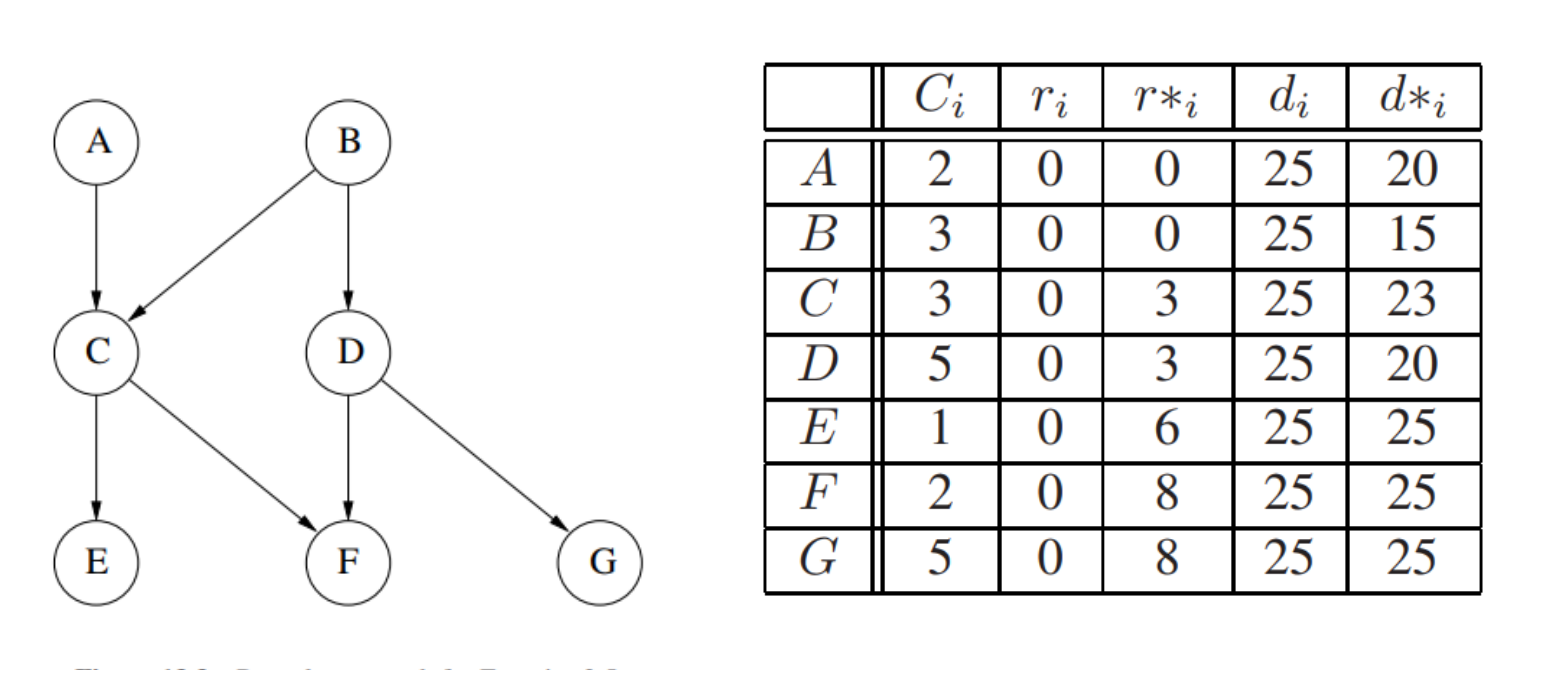
\includegraphics[scale=0.17]{pics/input1.png}

خروجی اول تولیدشده توسط کد 

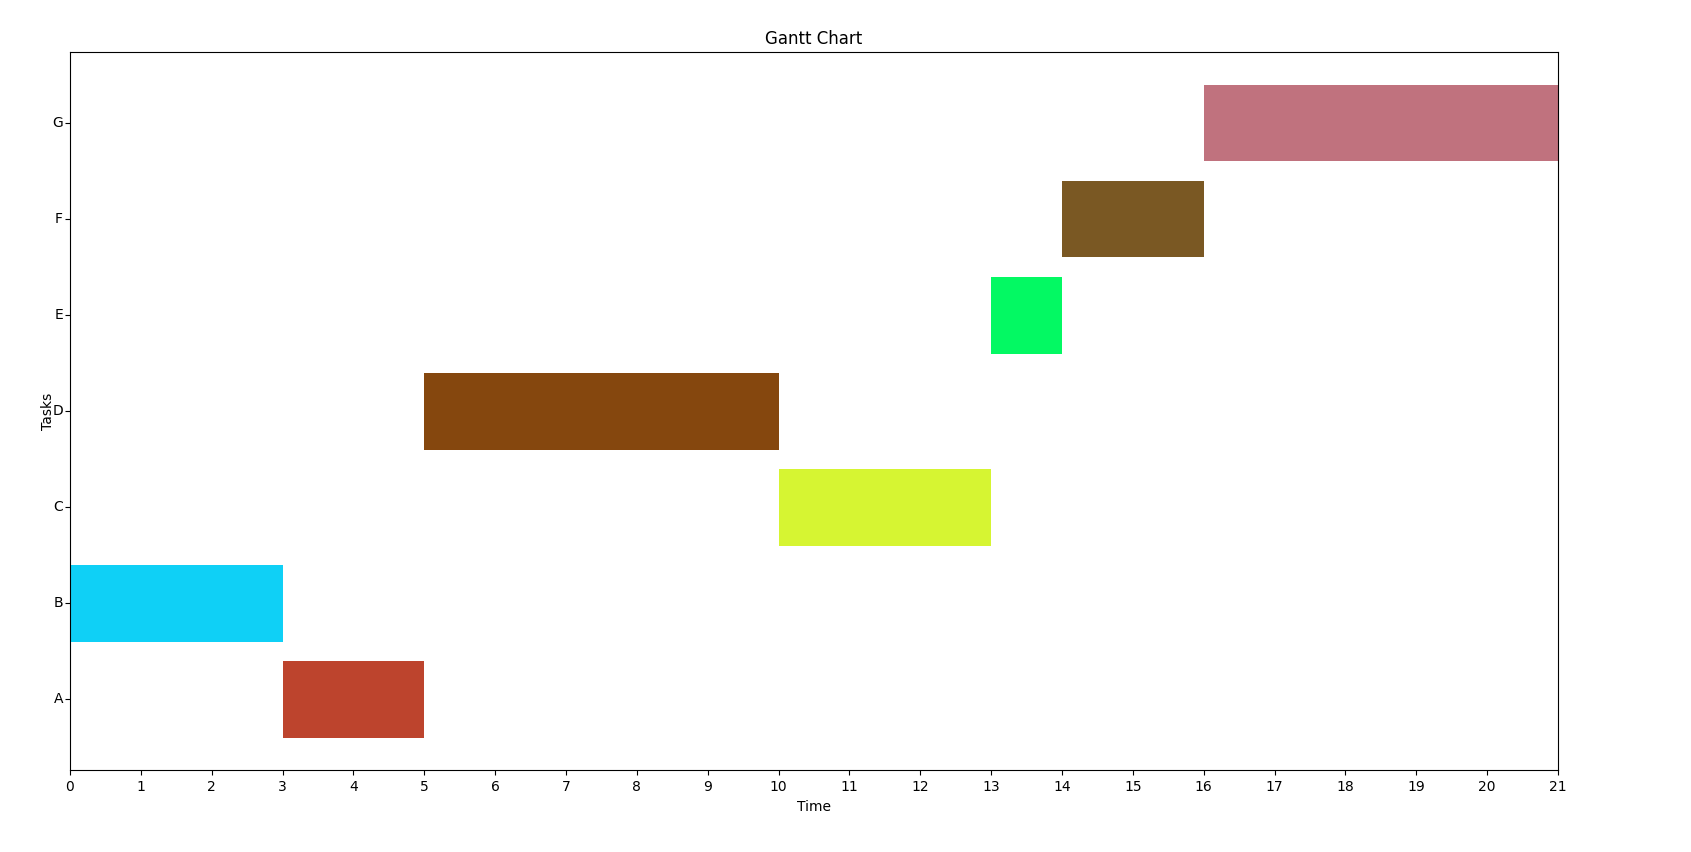
\includegraphics[scale=0.3]{pics/output1.png}

ورودی دوم : example\_tree2 

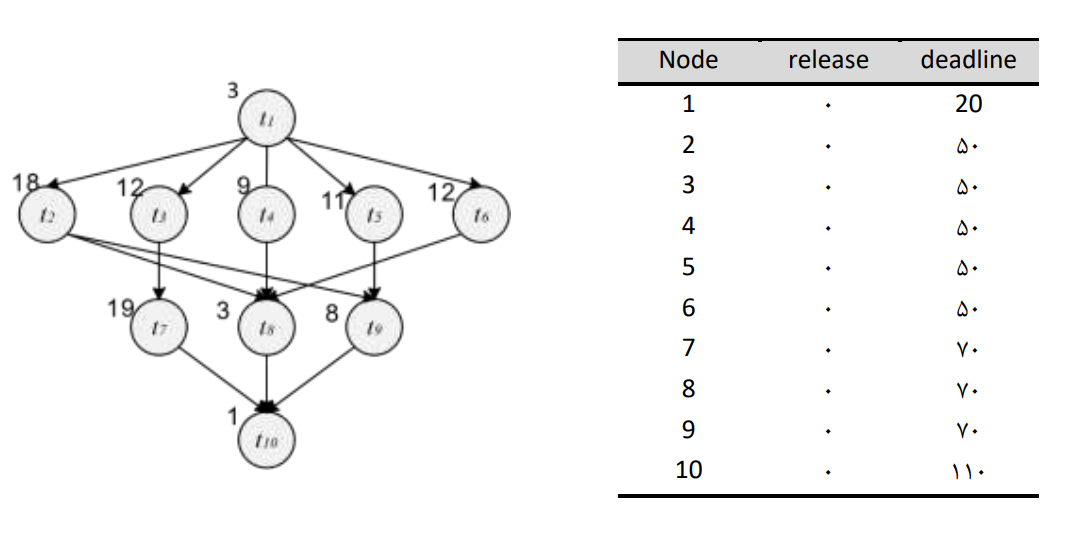
\includegraphics[scale=0.2]{pics/input2.png}

خروجی دوم تولید شده توسط کد که نشان می‌دهد این درخت قابل زمان‌بندی نیست و حداقل یکی از تسک‌ها ددلاینش را رد می‌کند.

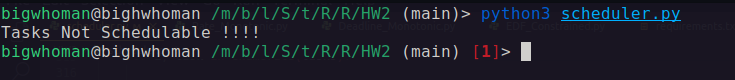
\includegraphics[scale=0.35]{pics/output2.png}

ورودی سوم : example\_tree3 

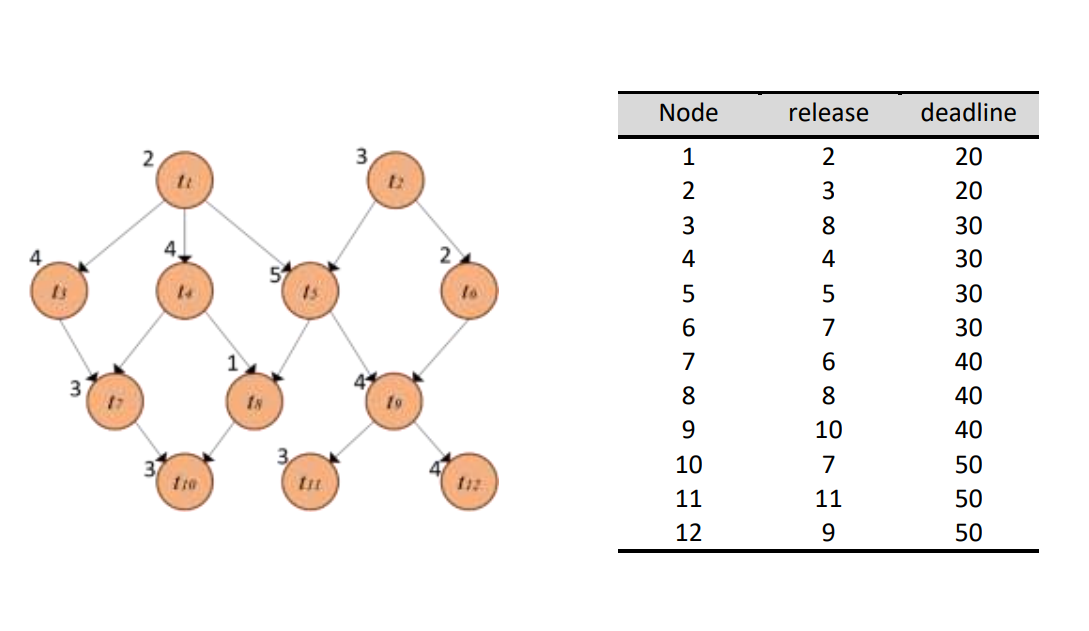
\includegraphics[scale=0.17]{pics/input3.png}

خروجی سوم تولید شده توسط کد 

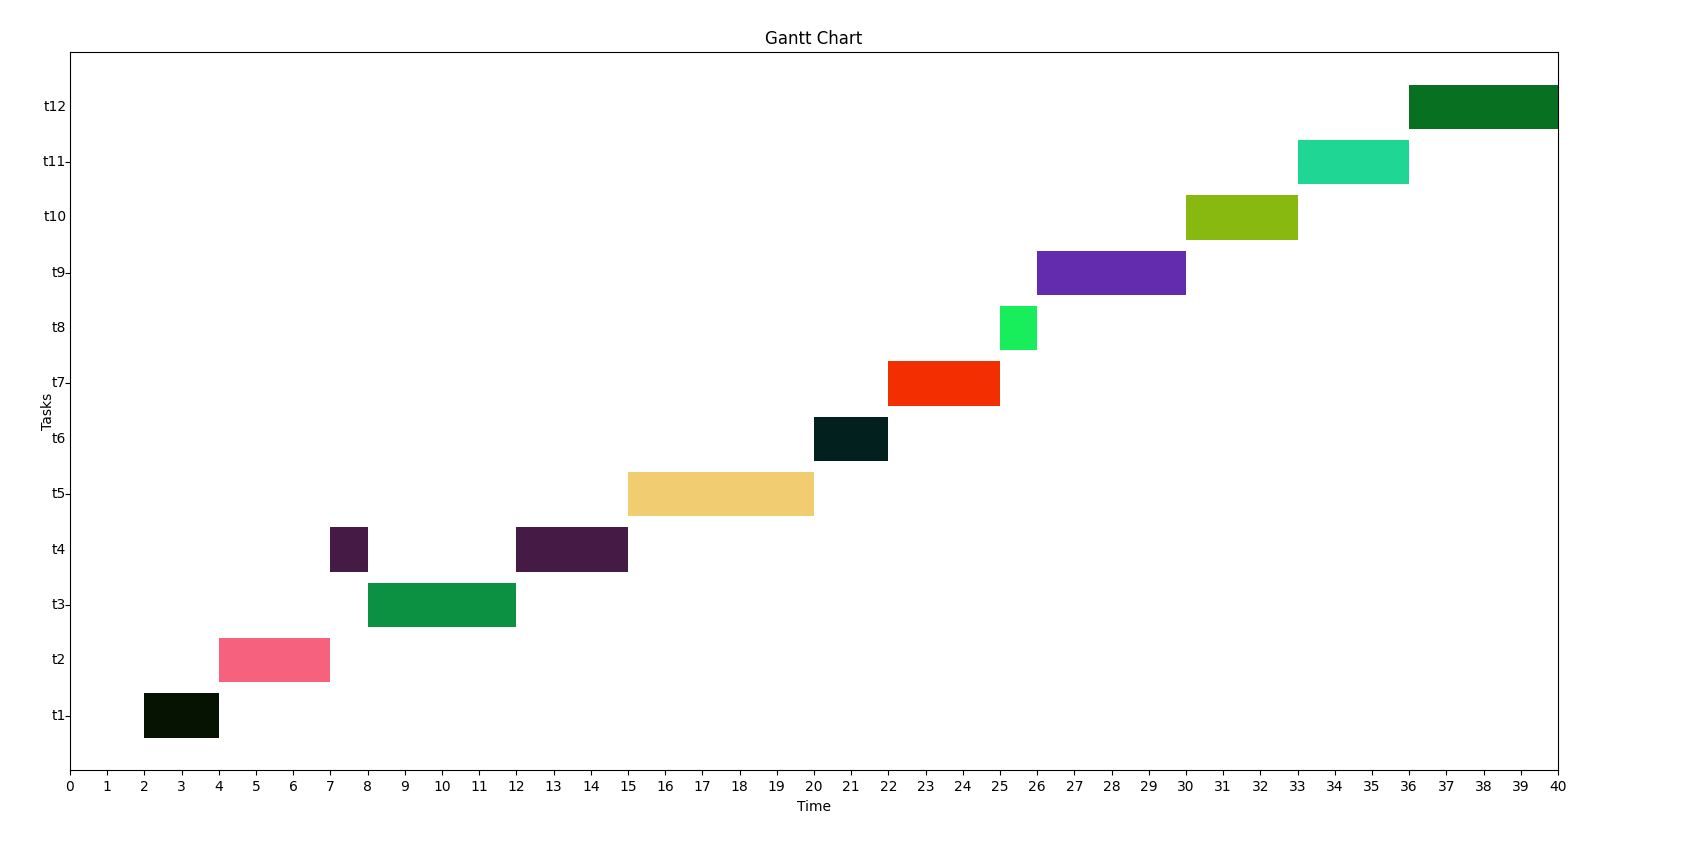
\includegraphics[scale=0.3]{pics/output3.png}